\begin{marginfigure}
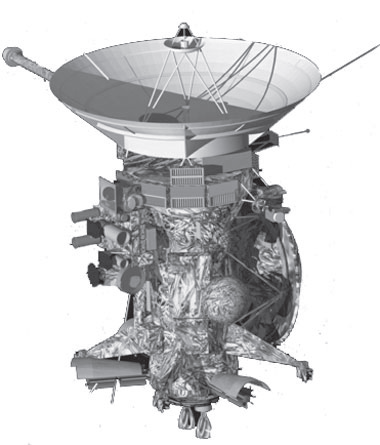
\includegraphics[width=\linewidth]{fig_00}
\end{marginfigure}

\subsection*{Activité préparatoire : Génération d'une grille -- Déjà fait sur Capytale}


Soit une grille rectangulaire $n\times p$ constituée de $n$ colonnes et de $p$ lignes contenant toutes les arêtes possibles. On modélise cette grille par un graphe dont l'ensemble des sommets est donné par les couples $(i,j)$ tels que : $i\in\llbracket 0,n \llbracket $ et $j\in\llbracket 0,p \llbracket $.

Les voisins d'un sommet $(i,j)$ sont ceux situés en haut, en bas, à droite et à gauche s'ils existent (par exemple, le sommet $(0,0)$ a comme voisin les sommets $(0,1)$ et $(1,0)$).



\begin{figure}[!h]\centering
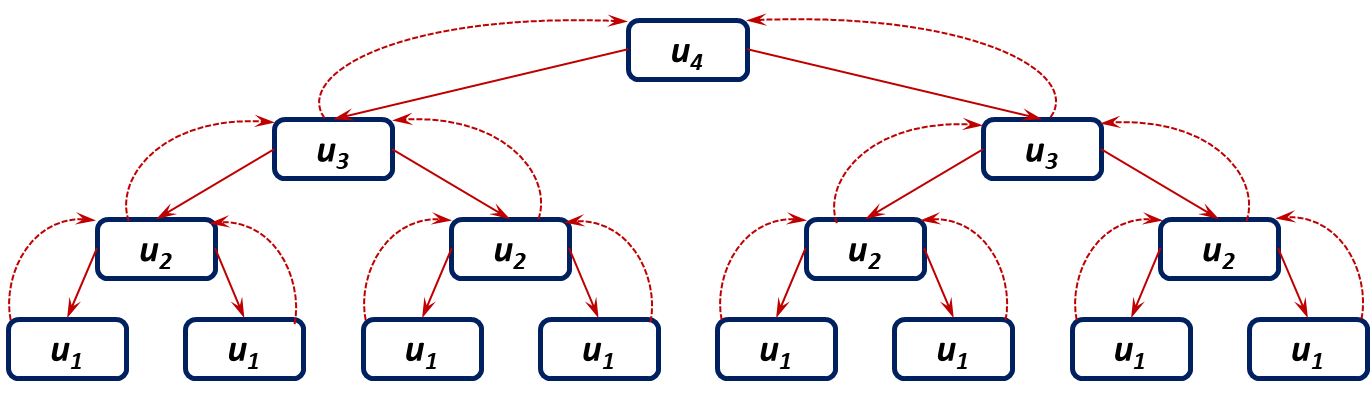
\includegraphics[width=12cm]{fig_01}
\caption{Grille (5,3) et grille (2,2)}
\end{figure}

Le graphe est implémenté par un dictionnaire d'adjacence où les clés sont les tuples, coordonnées d'un sommet. La valeur associée est une liste des sommets voisins. 


\begin{question}
Écrire la fonction \lstinline{creer_graphe(n:int, p:int) -> dict} permettant de créer le graphe d'une grille de \lstinline{n} colonnes et \lstinline{p} lignes.
\end{question}

\begin{exemple}
La grille $ 2 \times 2$ sera modélisée par le graphe suivant :

\begin{lstlisting}
>>> G2 =  creer_graphe(2,2)
>>> G2
        {(0, 0): [(1, 0), (0, 1)],
        (1, 0): [(1, 1), (0, 0)],
        (0, 1): [(1, 1), (0, 0)],
        (1, 1): [(0, 1), (1, 0)]}
\end{lstlisting}
\end{exemple}

On souhaite afficher ce graphe en utilisant \lstinline{matplotlib}. Pour cela, on va commencer par tracer chacune des arêtes puis chacun des sommets. 

\begin{question}Écrire la fonction \lstinline{get_sommets(G:dict) -> (list,list)} renvoyant deux listes \lstinline{les_x} et \lstinline{les_y} contenant respectivement les abscisses des sommets et les ordonnées des sommets.
\end{question}


\begin{exemple}
Dans l'exemple qui suit, les coordonnées de sommets peuvent être dans un ordre différent. 
\begin{lstlisting}
>>> les_sx, les_sy = get_sommets(G2)
>>> les_sx, les_sy
        ([0, 1, 0, 1], [0, 0, 1, 1])
\end{lstlisting}
\end{exemple}


\begin{question}
Écrire la fonction \lstinline{trace_sommets(G:dict, couleur : str) -> None} qui trace sur la figure courante les sommets en utilisant un point coloré.

Exemples : pour tracer avec des points rouge on utilise la fonction suivante : \lstinline{plt.plot(x,y,'r.')};  en bleu : \lstinline{plt.plot(x,y,'b.')}, en noir : \lstinline{plt.plot(x,y,'k.') }.
\end{question}

\begin{question}
Écrire la fonction \lstinline{get_aretes(G:dict) -> list} renvoyant la liste des arêtes du graphe sous la forme d'une liste de listes de tuples. Une arête est donc une liste de sommets où les sommets sont des tuples. Les arêtes ne devront être présentes qu'une fois.
\end{question}

\begin{exemple}
Dans l'exemple qui suit, l'ordre des arêtes peut être dans un ordre différent. Pour une arête donnée, les sommets peuvent aussi être dans un ordre différent.
\begin{lstlisting}
>>> get_aretes(G2)
	[[(0, 0), (1, 0)], [(0, 0), (0, 1)], [(1, 0), (1, 1)], [(0, 1), (1, 1)]]
\end{lstlisting}
\end{exemple}


\begin{marginfigure}\centering
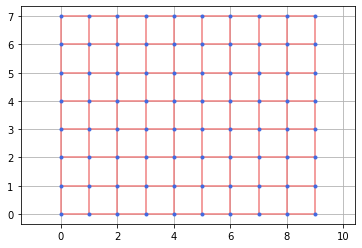
\includegraphics[width=\linewidth]{grille_10_8}
\caption{Tracé d'un graphe grille de 10 colonnes et 8 lignes}
\end{marginfigure}


\begin{question}
Écrire la fonction \lstinline{trace_arete(s1:tuple, s2:tuple, couleur : str , epaisseur : int ) -> None} qui trace une arête reliant les sommets \lstinline{s1} et \lstinline{s2} sur la figure courante. 

Exemple : pour tracer l'arête [(0,2),(1,2)] en bleu avec une épaisseur de 2, il faut utiliser l'instruction : \lstinline{plt.plot([0,1],[2,2],'b',linewidth=2)}.
\end{question}


\begin{question}
Écrire la fonction \lstinline{trace_graphe(G:dict,couleur : str,epaisseur : int) -> None} qui permet de tracer les sommets et les arêtes du graphe \lstinline{G} sur la figure courante. Tracer le graphe en rouge avec une épaisseur de 1 pour obtenir la figure ci-dessous.
\end{question}
